Here's some sample TikZ code that could generate an image similar to what you described:
```
\documentclass{standalone}
\usepackage{tikz}
\begin{document}
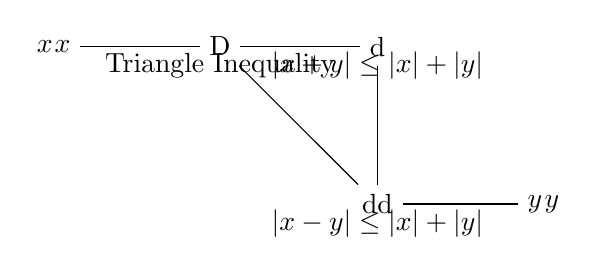
\begin{tikzpicture}[node distance=2cm]
  % Nodes
  \node (A) {D};
  \node (B) [right of=A] {d};
  \node (C) [below of=B] {dd};
  \node (X) [left of=A] {$x$};
  \node (Y) [right of=C] {$y$};
  
  % Lines
  \draw (A) -- (B);
  \draw (B) -- (C);
  \draw (C) -- (A);
  \draw (A) -- (X);
  \draw (C) -- (Y);
  
  % Equations
  \node at (A.south) {Triangle Inequality};
  \node at (B.south) {$|x+y|\leq |x|+|y|$};
  \node at (C.south) {$|x-y|\leq |x|+|y|$};
  \node at (X.west) {$x$};
  \node at (Y.east) {$y$};
\end{tikzpicture}
\end{document}
```
This code creates a simple diagram with three nodes labeled "D," "d," and "dd," connected by lines to form a triangle. It also includes labels for the variables "x" and "y" and the triangle inequality equation in three different forms. You can modify this code to add more details and customize the appearance of the diagram to better match your specific needs.